% ---------------------------------------------------------------------
% HEADER
% Formålet med å legge header til et eget dokument er å garantere at
% oppsettet av dokumentene er likt for alle løsningsforslagene.
% I headeren skjer følgende:
% (1) Dokumentet blir startet
% (2) Pakker blir importert
% ---------------------------------------------------------------------
% ---------------------------------------------------------------------
% HEADER
% Formålet med header er å importere de samme pakkene i alle dokumentene.
% ---------------------------------------------------------------------

% Sett opp dokumentet. Her kan 'twoside' brukes for printing
\documentclass[12pt, a4paper]{article}

% Vi trenger utf-8 for å bruke norske bokstaver: Æ, Ø, Å
\usepackage[utf8]{inputenc}

% Vi setter babel til norsk, da får dokumentegenskaper norske titler
\usepackage[norsk]{babel}

% For å kunne bruke grafikk
\usepackage{graphicx}
\newcommand{\figwidth}{0.75}

% Matematikkpakker fra AMS - American Mathematical Society
\usepackage{amsmath, amsthm, amsfonts, amssymb, mathtools}

% For eventuelle linker, e.g. \href{URL}{text}
\usepackage{hyperref}

% For headers og footers med eventuell logo
\usepackage{fancyhdr}

% Sett marginer manuelt
\usepackage[top = 3cm, left = 3cm, right = 3cm, bottom = 3cm]{geometry}

% For enkle lister, nyttig for oppgave a), b), c), ...
\usepackage[sharp]{easylist}

% Dersom flere kolonner er ønskelig i deler av dokumentet
\usepackage{multicol}

% For luft mellom paragrafer
\usepackage{parskip}

% For logikk assosiert med logoer
\usepackage{ifthen}

% For å finne totalt antall sider
\usepackage{lastpage}

% Annet
\usepackage{enumitem}

\usepackage{polynom}% Polynomer
\polyset{style=C, div=:}

\usepackage{systeme}% Likningssystemer

% Kan brukes når noe stryker ut noe, f.eks 1/n * n, her kan man ta \frac{1}{\cancel{n}} * \cancel{n}
\usepackage{cancel}



% ---------------------------------------------------------------------
% DOKUMENTVARIABLER
% ---------------------------------------------------------------------
\newcommand{\fagkode}{R1}
\newcommand{\semesteraar}{høsten 2018}
\newcommand{\forfatter}{Tommy O.}
\newcommand{\dokumenttittel}{Løsningsforslag -- Eksamen \fagkode, \semesteraar}

\usepackage{siunitx}


% Set til 'true' og oppgi logo dersom du vil bruke en logo
\newboolean{bruklogo}
\setboolean{bruklogo}{false}
\newcommand{\logonavn}{}



% ---------------------------------------------------------------------
% SETUP
% Formålet med å legge setup til et eget dokument å garantere at headers,
% footers, og øverste del av dokumentet er likt for alle
% løsningsforslagene.
% ---------------------------------------------------------------------
% ---------------------------------------------------------------------
% HEADER
% Formålet med setup er at dokumentene ser rimelig like ut.
% ---------------------------------------------------------------------


% ---------------------------------------------------------------------
% Alternativ font. Kommentert ut fordi Computer Modern (default) er pen
%\usepackage{kmath,kerkis}
%\usepackage[T1]{fontenc}
% ---------------------------------------------------------------------


% ---------------------------------------------------------------------
% Sett opp headers og footers
\ifthenelse{\boolean{bruklogo}}{
% Dersom logo skal brukes, sett logoen oppe til høyre med bredde 4 cm
	\rhead{\includegraphics[width=3.5cm]{\logonavn}}
}{
% Dersom logo ikke skal brukes, sett tom header
	\rhead{}
} 
\rfoot{\thepage}
\cfoot{}
\lhead{}
\lfoot{{\scriptsize Forbedringsforslag? Bidra på \url{https://github.com/tommyod/matte_eksamener_VGS}.}}
\renewcommand{\headrulewidth}{0pt}
% ---------------------------------------------------------------------


% ---------------------------------------------------------------------
% To streker under svaret
\def\answer#1{\underline{\underline{#1}}}
% ---------------------------------------------------------------------


% ---------------------------------------------------------------------
% Start selve dokumentet
% ---------------------------------------------------------------------

\begin{document}
\pagestyle{fancy}
{\bfseries \Large \dokumenttittel} \\
{ \footnotesize Laget av \forfatter 
	\hfill Sist oppdatert: \today 
	\hfill Antall sider: \pageref*{LastPage}}
\hrule
\vspace{1em}
\begin{center}
\fbox{\fbox{\parbox{.90\textwidth}{
	Dette dokumentet er open-source;
	alle kan bidra til å gjøre det bedre.
	Dersom du finner skrivefeil, matematiske feil, eller ser at forklaringene kan være bedre: ikke nøl med å sende inn en endring. 
	Du kan finne siste versjon, og bidra, på GitHub, se:
	\url{https://github.com/tommyod/matte_eksamener_VGS}
}}}
\end{center}


% ---------------------------------------------------------------------
% DOKUMENTSTART - Skriv løsningsforslaget nedenfor
% ---------------------------------------------------------------------	
\section*{Del 1 - uten hjelpemidler}
\subsection*{Oppgave 1}
\begin{easylist}[enumerate]
	\ListProperties(Style2*=,Numbers=a,Numbers1=l,FinalMark={)})
	# sdf
	# sdf
	# sdf
\end{easylist}


\subsection*{Oppgave 2}
\begin{easylist}[enumerate]
	\ListProperties(Style2*=,Numbers=a,Numbers1=l,FinalMark={)})
	# sdf
	# sdf
\end{easylist}

\subsection*{Oppgave 3}
\begin{easylist}[enumerate]
	\ListProperties(Style2*=,Numbers=a,Numbers1=l,FinalMark={)})
	# sdf
	# sdf
	# sdf
\end{easylist}


\subsection*{Oppgave 4}
\begin{easylist}[enumerate]
	\ListProperties(Style2*=,Numbers=a,Numbers1=l,FinalMark={)})
	# sdf
	# sdf
	# sdf
\end{easylist}


\subsection*{Oppgave 5}
\begin{easylist}[enumerate]
	\ListProperties(Style2*=,Numbers=a,Numbers1=l,FinalMark={)})
	# sdf
	# sdf
\end{easylist}


\subsection*{Oppgave 6}
asdf


\subsection*{Oppgave 7}
\begin{easylist}[enumerate]
	\ListProperties(Style2*=,Numbers=a,Numbers1=l,FinalMark={)})
	# sdf
	# sdf
	# sdf
\end{easylist}


\subsection*{Oppgave 8}
\begin{easylist}[enumerate]
	\ListProperties(Style2*=,Numbers=a,Numbers1=l,FinalMark={)})
	# sdf
	# sdf
	# sdf
\end{easylist}







\clearpage 
\section*{Del 2 - med hjelpemidler}


\subsection*{Oppgave 1}
La $X$ være antall gule blomster.
Da er $X$ binomisk fordelt, fordi fargen til hver blomst er uavhengig av de andre, sannsynligheten for gul er alltid $p = 0.4$, og det er kun to utfall per blomst---enten gul eller rød.

\begin{easylist}[enumerate]
	\ListProperties(Style2*=,Numbers=a,Numbers1=l,FinalMark={)})
	# Vi lar $X$ være antall gule blomster, da er $X$ binomisk fordelt med $n=10$ og $p=0.4$. 
	Sannsynligheten for at $X=5$ blir da
	\begin{equation*}
		P(X = 5) = \binom{n}{k} p^k (1-p)^{n-k} = 
		\binom{10}{5} 0.4^5 0.6^{5} \approx 0.2007 = \answer{20.1 \, \%},
	\end{equation*}
	der vi henter svaret fra Geogebras sannsynlighetskalkulator i praksis.
	# Dette er $P(X > 5)$, og fra sannsynlighetskalkulatoren i Geogebra får vi
	\begin{equation*}
		P(X > 5) \approx 0.1662 = \answer{16.6 \, \%} .
	\end{equation*}
	# Her kan det være nyttig å snu litt på problemstillingen.
	Vi har 10 plasser $P_1, P_2, \dots, P_{10}$ totalt, og vi må trekke ut fire plasser til de gule blomstene.
	Da er plasseringen til de andre blomstene også bestemt.
	Rekkefølgen har ikke noe å si, fordi $\{ P_3, P_5, P_6, P_9 \}$ eksempelvis er det samme som $\{ P_6, P_5, P_3, P_9 \}$.
	Spørsmålet er med andre ord ``På hvor mange måter kan vi velge 4 plasser for de gule blomstene, nå rekkefølgen er uviktig?''.
	Dette er antall kombinasjoner, og svaret blir $\binom{10}{4} = \answer{210}$.
	I Geogebra skriver man \verb|nCr(10, 4)| i CAS.
	
	Legg også merke til at dette spørsmålet er det samme som å spørre ``På hvor mange måter kan vi velge 6 plasser for de røde blomstene, nå rekkefølgen er uviktig?'', og at svaret da blir $\binom{10}{6} = \answer{210}$.
\end{easylist}

\subsection*{Oppgave 2}
\begin{easylist}[enumerate]
	\ListProperties(Style2*=,Numbers=a,Numbers1=l,FinalMark={)})
	# sdf
	# sdf
	# sdf
	# sdf
	# sdf
\end{easylist}



\subsection*{Oppgave 3}
\begin{easylist}[enumerate]
	\ListProperties(Style2*=,Numbers=a,Numbers1=l,FinalMark={)})
	# Linjen $\ell$ er gitt av
	\begin{equation*}
		\ell(k) = A + \vec{AB} k = (3, 0) + \left[ (5, 5) - (3, 0) \right] k = (2k+3, 5k).
	\end{equation*}
	# Se figur \ref{fig:del2_oppg3} for en tegning av grafen, utført med kommandoen \\
	\verb|Kurve(<Uttrykk>, <Uttrykk>, <Parametervariabel>, <Start>, <Slutt>)|,\\
	samt linjen $\ell(k)$.
	# Linja fra $A$ til $B$ er gitt av $\vec{AB} = (2, 5)$.
	Tangenten er gitt av $T(t) = r'(t) = (1, 2t)$.
	Disse to vektorene er paraelelle dersom der finnes en $z$ slik at
	\begin{equation*}
		\begin{pmatrix}
		2 \\
		5
		\end{pmatrix} z =
		\begin{pmatrix}
		1 \\
		2t
		\end{pmatrix}.
	\end{equation*}
	Dette er et likningssett med 2 ukjente og 2 likninger, og løsningen er $z = 1/2$ og $t = 5/4$.
	Setter vi $t = 5/4$ inn i $r(t)$ får vi punktet 
	\begin{equation*}
		\answer{\begin{pmatrix}
			9/4 \\
			57/6
			\end{pmatrix}},
	\end{equation*}
	og dette er punktet på $r(t)$ som er nærmest $\ell$.
\end{easylist}

\begin{figure}[ht!]
\centering
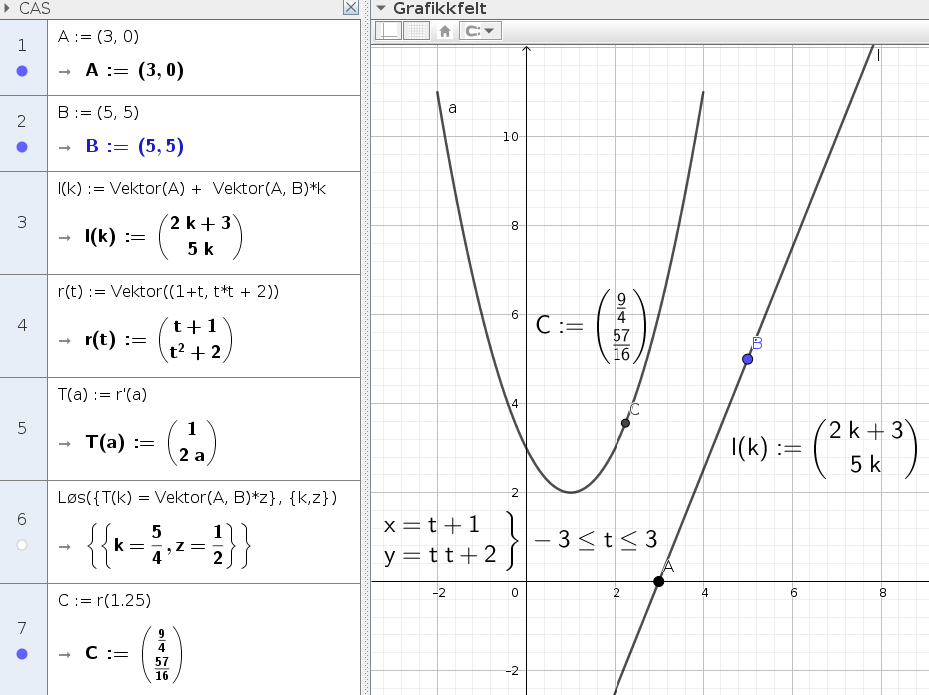
\includegraphics[width=0.9\linewidth]{figs/del2_oppg3}
\caption{Løsning på oppgave 3, del 2.}
\label{fig:del2_oppg3}
\end{figure}

\subsection*{Oppgave 4}
\begin{easylist}[enumerate]
	\ListProperties(Style2*=,Numbers=a,Numbers1=l,FinalMark={)})
	# Se figur \ref{fig:del2_oppg4_a}.
	
	\begin{figure}[ht!]
	\centering
	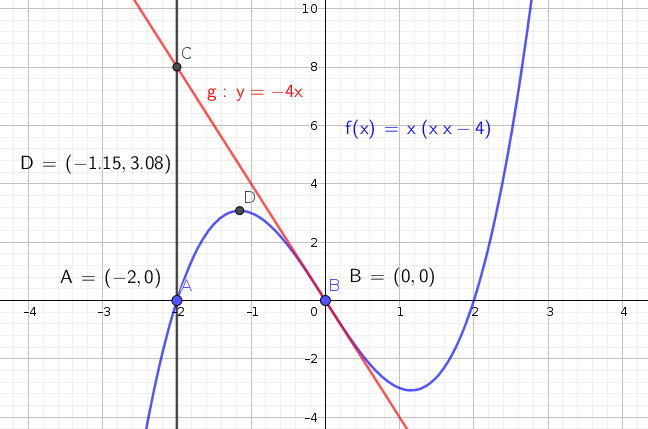
\includegraphics[width=0.9\linewidth]{figs/del2_oppg4_a}
	\caption{Løsning på oppgave 4a, del 2.}
	\label{fig:del2_oppg4_a}
	\end{figure}
	
	# Der bruker vi \verb|Mangekant(A, B, C) / Mangekant(A, B, D)| og får $2.5981 \approx \answer{2.6}$ som svar.

	# sdf
\end{easylist}





\end{document}